\section{Application side} 
    
    Before delving deeper into the parts, we present the global system design diagram. We recognise two separate parts.
    \begin{itemize}
        \item The application side, where the Erlang system under test is. Consequently, it's where the $\Delta$Q adapter will be, which performs the translation of spans to outcome instances.
        \item The oscilloscope side, where the $\Delta$Q oscilloscope receives information from the adapter attached to the system under test to display graphs, define outcome diagrams and set parameters for probes.
    \end{itemize}

    \begin{figure}[H]
        \begin{center}
            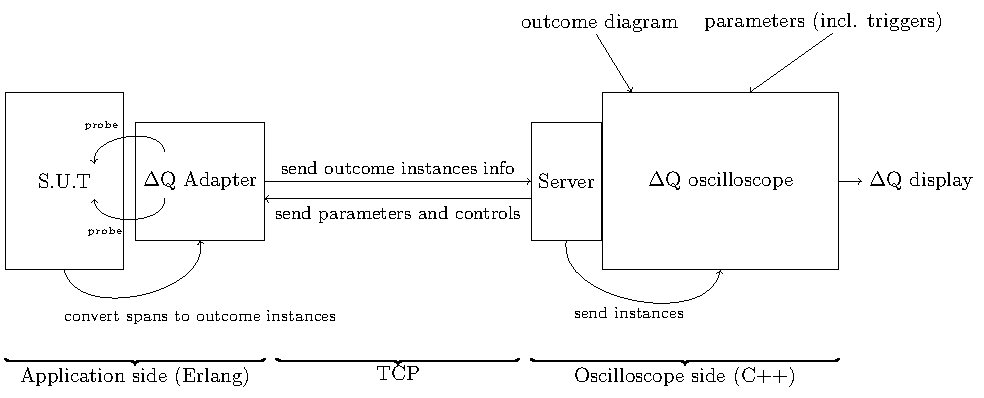
\includegraphics[width=\textwidth]{tikz/sut-stub-osc.pdf}
        \end{center}
        \caption{Global system design diagram.}
    \end{figure}


    \subsection{System under test} The system under test \textbf{(S.U.T)} is the Erlang system the engineer wishes to observe, it ideally is a system which already is instrumented with OpenTelemetry. The ideal system where $\Delta$QSD is more useful is a system that executes many independent instances of the same action \cite{dq-tut}. 
    
    \subsection{$\Delta$Q Adapter} The $\Delta$Q adapter is the \texttt{dqsd\_otel} Erlang application \cite{wrapper}, it starts and ends OpenTelemetry spans and translates them to outcome instances which are useful for the oscilloscope. This can be done thanks to probes being attached to the system under test, like an oscilloscope would! The outcome instances end normally like OpenTelemetry spans or, additionally, can timeout, given a custom timeout ($dMax$), and fail, \textit{according to user's definition of failure}. 
    
    Handling of OpenTelemetry spans which goes beyond starting and ending them is delegated to the user, who may wish to do further operations with their spans. 
    The adapter is called from the system under test and communicates outcome instances data to the oscilloscope via TCP. 
    
    The adapter can receive messages from the oscilloscope, the messages are about updating probe's $dMax$ or starting and stopping the sending of data to the oscilloscope.
    \subsection{Inserting probes in Erlang - From spans to outcome instances}
        OpenTelemetry spans are useful to carry context, attributes and baggage in a program. The plethora of attributes they have is nevertheless too much for the oscilloscope. \cite{otel-dt}

        To get the equivalent of spans for the oscilloscope, the adapter needs to be called at the starting events of a probe to start an instance of a probe, and at the ending events to end the outcome instance. The name given with \texttt{"start\_span"} is the name of the probe.

     
\begin{figure}[!ht]
\centering
   \begin{minted}{erlang}
        % Start the outcome instance of probe. The call to dqsd_otel starts an OpenTelemetry span, as it contains a call to ?start_span(Name)
        {ProbeCtx, ProbePid} = dqsd_otel:start_span(<<"probe">>),  

        % Start and fail span directly
        {WorkerCtx, WorkerPid} = dqsd_otel:start_span(<<"worker_1">>),   
        dqsd_otel:fail_span(WorkerPid),
        %Here, you would need to end the span manually with ?end_span

        %Example of with_span, the call to OpenTelemetry ?with_span is inside the adapter function, the function fun() -> ok end is executed inside dqsd_otel.
        dqsd_otel:with_span(<<"worker_2">>, fun() -> ok end), 
        %End the outcome instance of probe. This ends the OpenTelemetry span aswell. If the outcome instance has already timed out (the time from start_span to end_span > dMax), the oscilloscope receives no message where the status is successful. Otherwise, this sends a message with startTime, endTime, the name "probe" and success status.
        dqsd_otel:end_span(ProbeCtx, ProbePid),
        \end{minted}
\caption{Example usage of the adapter}\label{code:adapter}
\end{figure}
    Further details about the implementation of the adapter are explained in the following chapters. 
